 . .
\documentclass{article}
\usepackage[utf8]{inputenc}
\usepackage{blindtext}
\usepackage{graphicx}
\usepackage{amsmath}
\usepackage{csvsimple}
\usepackage{pdfpages}
\usepackage{hyperref}
\usepackage{gensymb}

\begin{document}
\begin{center}
\textbf{\Huge{University of South Bohemia}}\\
\vspace{50px}
\textbf{\Large{Faculty of Science}} \\
\vspace{30px}
\includegraphics[width=120px]{~/school/logo.png} \\
\vspace{30px}
\textbf{\large{Praktika IV}}
\vspace{20px}
\\
\vspace{20px}
\large{Frank-Hertzův experiment} \\
\vspace{60px}
\end{center}
\begin{flushleft}
Datum: 18.10.2023 \\
Jmeno: Martin Skok \\
Obor: Fyzika \\
Hodnoceni:
\end{flushleft}
\newpage
\section{Úkoly}
Změřte závislost magnetického pole na rezonanční frekvenci vzorku DPPH (radikál 2,2-difenyl-1-pikrylhydrazylu) \\
Určete jeho $g$ faktor.
\section{Seznam pomůcek}
Počítač, 3B-NET log, 3B-NET lab program, jednostka s cívkami a se sondou, vzorek DPPH
\section{Teorie}
\section{Postum měření}
Sestavil jsem a zapnul obvod\\
Vložil jsem vzorek DPPH\\
Zapnul jsem počítač a spustil program 3B-NET lab\\
Nastavil jsem potřebné paratemry a spustil osciloskop\\
Nastavil jsem frekvenci na $40 MHz$ a uložil data\\
Toto jsem opakoval do frekvence kolem $80 Mhz$ po intervalech kolem $5Mz$\\
Frekvence jsem ne vždy dokázal nastavit na přesnou hodnotu, tak jsem si vždy zapsal aktualňí hodnotu frekvence\\
\section{Naměřená data}
\begin{figure}[!h]
  \hspace*{-10em}
  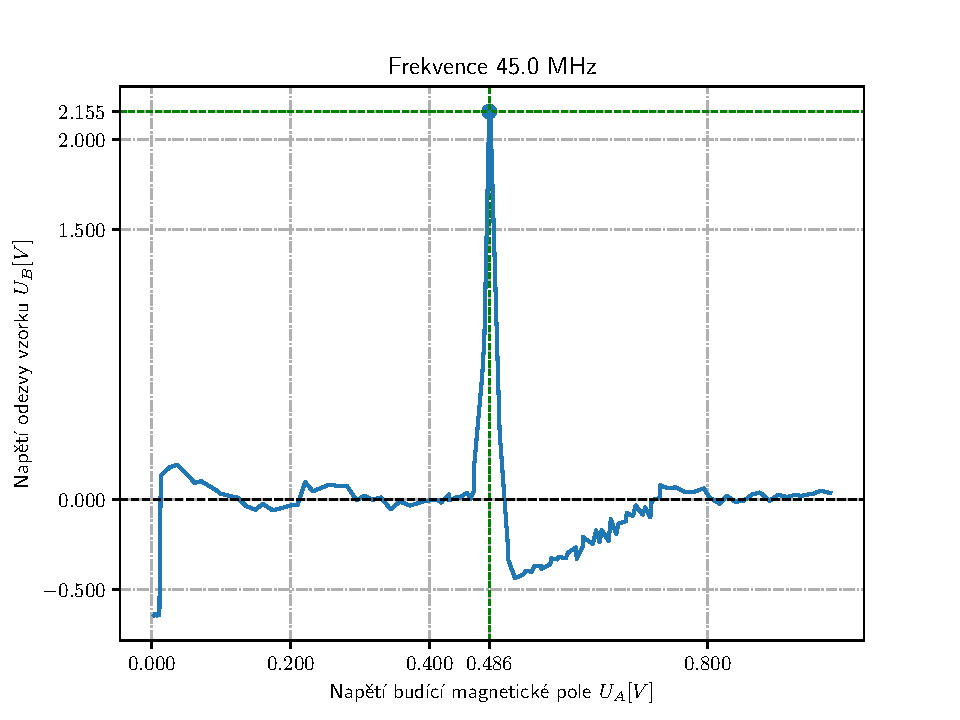
\includegraphics[scale=1.2]{figs/1.pdf}
  \caption{Graf závislosti napětí odezvy vzorku na napětím budícím magnetické pole}
\end{figure}
\begin{figure}[!h]
  \hspace*{-10em}
  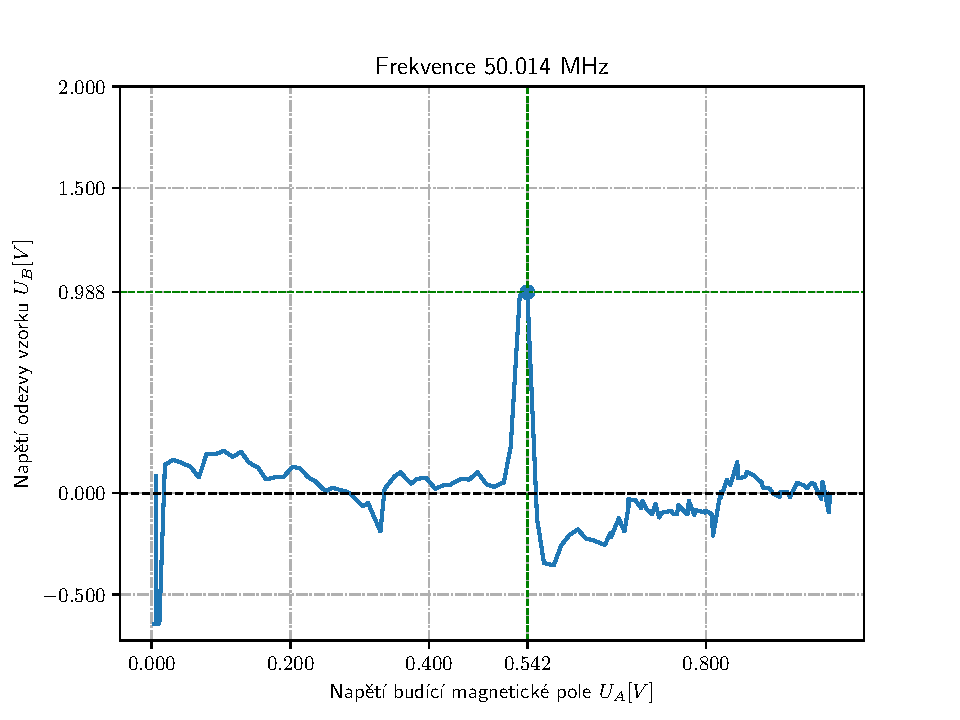
\includegraphics[scale=1.2]{figs/2.pdf}
  \caption{Graf závislosti napětí odezvy vzorku na napětím budícím magnetické pole}
\end{figure}
\begin{figure}[!h]
  \hspace*{-10em}
  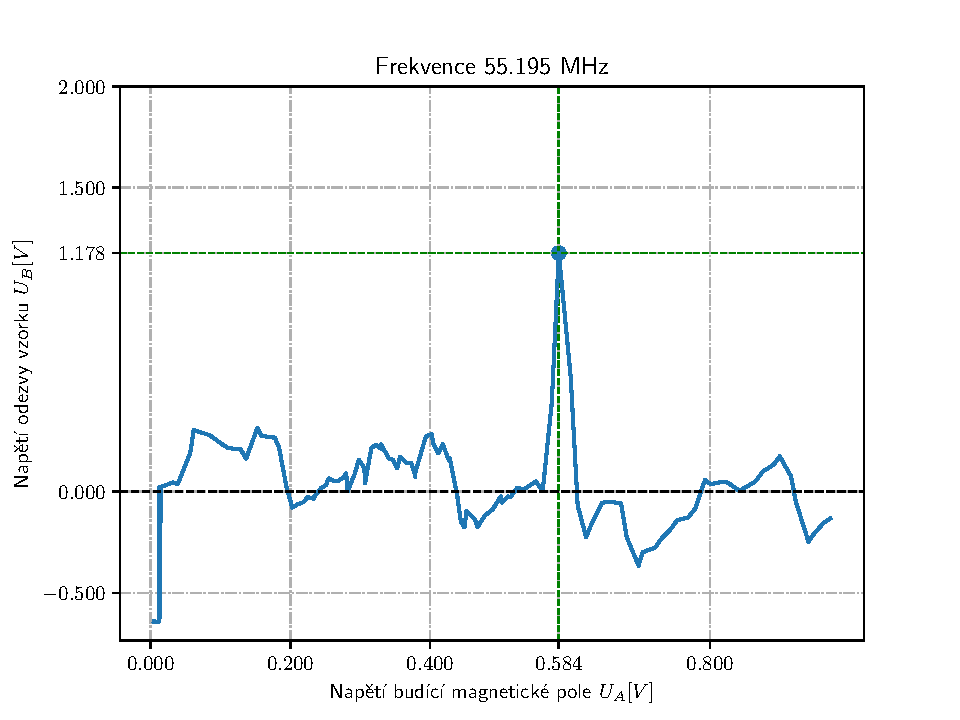
\includegraphics[scale=1.2]{figs/3.pdf}
  \caption{Graf závislosti napětí odezvy vzorku na napětím budícím magnetické pole}
\end{figure}
\begin{figure}[!h]
  \hspace*{-10em}
  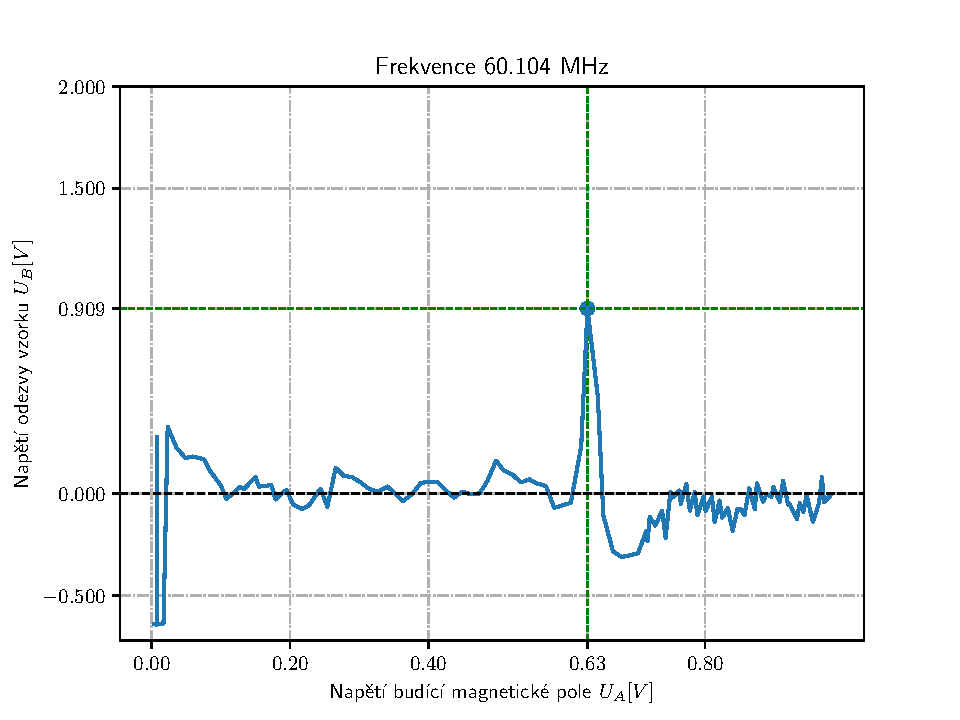
\includegraphics[scale=1.2]{figs/4.pdf}
  \caption{Graf závislosti napětí odezvy vzorku na napětím budícím magnetické pole}
\end{figure}
\begin{figure}[!h]
  \hspace*{-10em}
  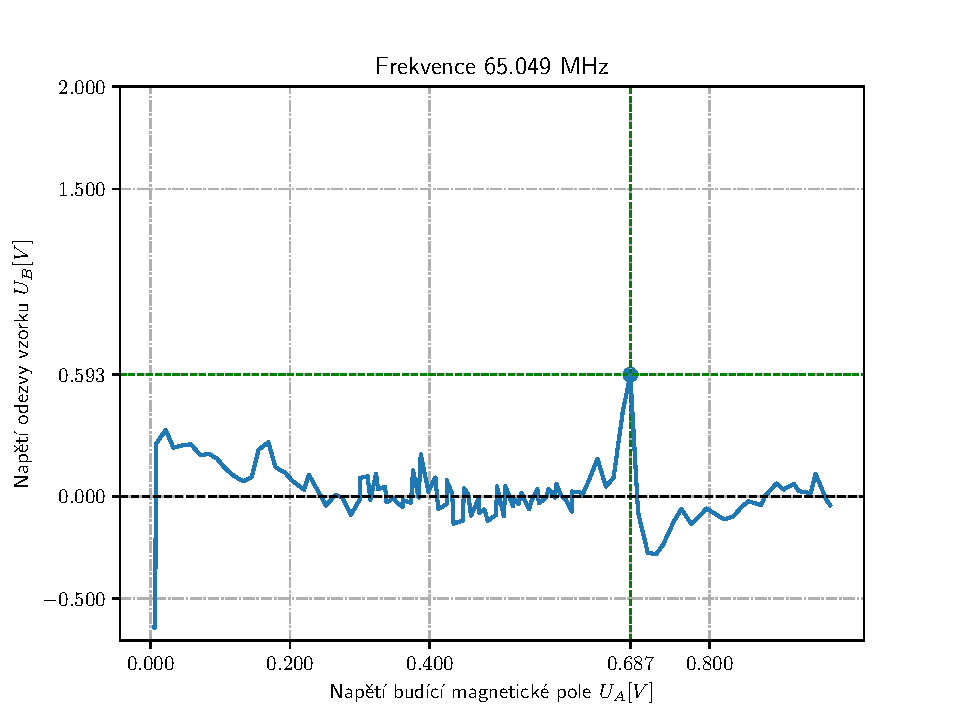
\includegraphics[scale=1.2]{figs/5.pdf}
  \caption{Graf závislosti napětí odezvy vzorku na napětím budícím magnetické pole}
\end{figure}
\begin{figure}[!h]
  \hspace*{-10em}
  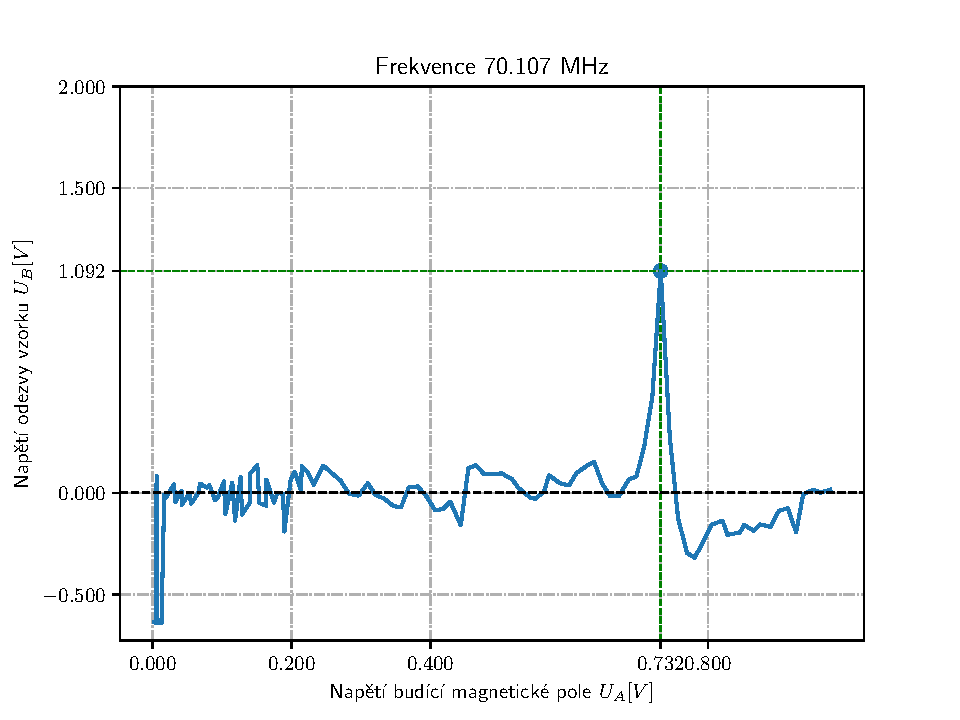
\includegraphics[scale=1.2]{figs/6.pdf}
  \caption{Graf závislosti napětí odezvy vzorku na napětím budícím magnetické pole}
\end{figure}
\begin{figure}[!h]
  \hspace*{-10em}
  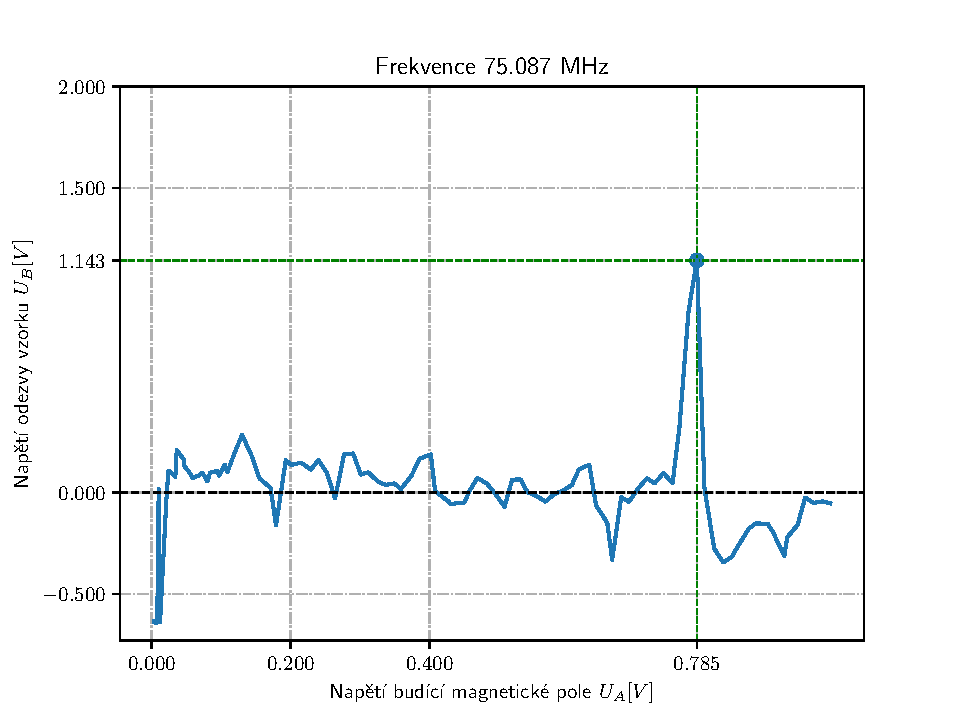
\includegraphics[scale=1.2]{figs/7.pdf}
  \caption{Graf závislosti napětí odezvy vzorku na napětím budícím magnetické pole}
\end{figure}
\begin{figure}[!h]
  \hspace*{-10em}
  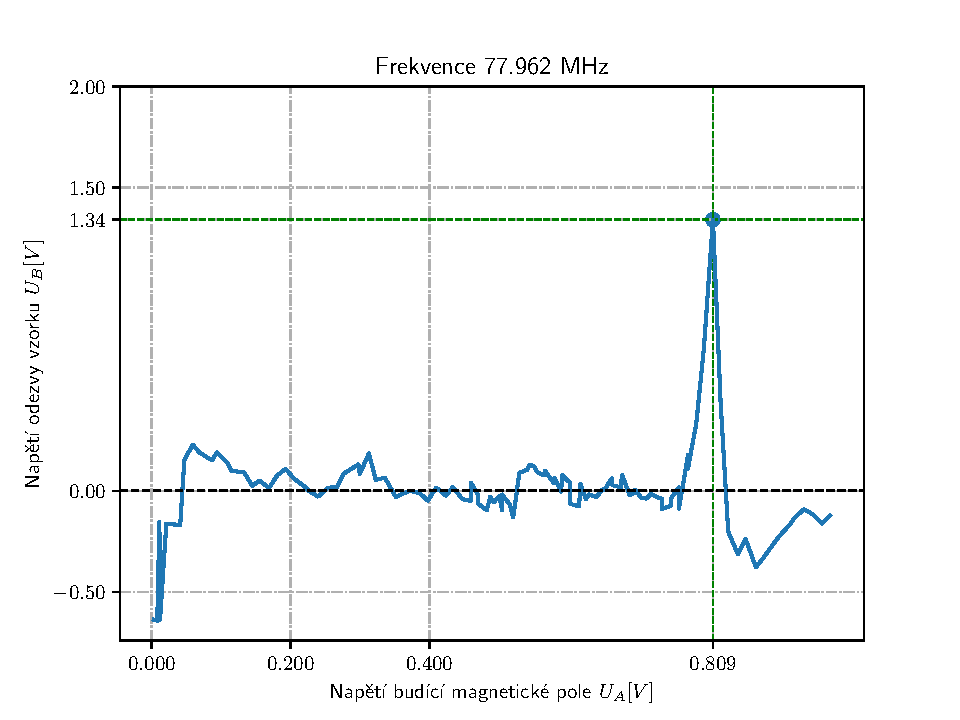
\includegraphics[scale=1.2]{figs/8.pdf}
  \caption{Graf závislosti napětí odezvy vzorku na napětím budícím magnetické pole}
\end{figure}
\end{document}
